We present the integration of Jupyter Notebooks into the MathHub system.

\subsection{Overview}

Our system consists of four components:
\begin{compactitem}
\item A GitLab repository hosting server \url{https://gl.mathhub.info} that provides persistent storage of documents in any format, including their OMDoc representation.
\item A Jupyter Notebook server \url{https://jupyter.mathhub.info} provides web-based IDE for editing interactive documents
\item An MMT instance which uses the OMDoc representations to provides the shared knowledge space and provides a high-level API for it\footnote{
    Technically, each kernel has a separate MMT instance in addition to the primary one. 
    Except for the ephemeral document representing each Notebook, these are identical to the main instance. 
    These exist only to isolate different users from one another, and prevent scenarios where they could unintentionally break each others notebook sessions.  
  }.
\item The MathHub frontend \url{https://mathhub.info} that serves as the main entry point and delegates some subtasks to the former.
  We have extended MathHub front-end with a new new document type presenter for notebooks that gives access to the source, context, statistics, and metadata of notebooks, and provides a ``preview'' and ``interact inline'' views.  
\end{compactitem}

The Jupyter server is an out of the box installation of Jupyter except for additionally supporting our new MMT kernel and a small plugin enabling smoother opening of notebooks via a url. 
Consequently, the integration between the Jupyter and the MathHub frontends is shallow: MathHub opens Jupyter Notebooks in separate tabs or iframes using URLs served by Jupyter.
A deeper integration -- e.g., using Jupyter simply as a JavaScript library in MathHub -- would have been preferable, but is infeasible because Jupyter is primarily designed as a monolithic system.
Recent versions of Jupyter are working Jupyter-as-a-module, so we leave deep integration to future work.

\subsection{Notebooks as Parts of Semantic Documents}

To interact dynamically with content in arbitrary MathHub documents, we can make use of the active computation widget presented in Section~\ref{sec:kernel:widgets}. 
For this purpose we implemented a new feature that creates a new ephemeral Jupyter Notebook and allows accessing it from the current document. 
Importantly, the new Notebook is pre-filled with an import of the current context. 

\begin{figure}[h]
  \begin{minipage}[c]{4cm}
  \vspace{-20pt}
  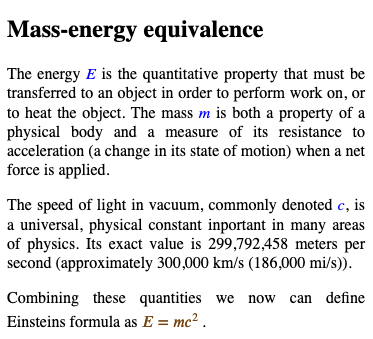
\includegraphics[width=4cm]{screenshots/sciencedoc}
  \end{minipage}
  \begin{minipage}[c]{7cm}
    \lstset{
  basicstyle=\small\ttfamily,
  columns=fullflexible,
  showstringspaces=false,
  commentstyle=\color{gray}\upshape,
  morestring=[b]",
  morestring=[s]{>}{<},
  morecomment=[s]{<?}{?>},
  stringstyle=\color{black},
  identifierstyle=\color{blue},
  keywordstyle=\color{cyan},
}
\begin{lstlisting}
<h2>Mass-energy equivalence</h2>
<div data-theory="?EEC">
 <p>
  The energy <span data-declares="E">E</span>
  The speed of light in vacuum ... 
  <span data-declares="c">c</span> ...
 </p>
 <p>
  We can now define Einsteins formula as 
  <math data-decls="m,c" data-uri="?E">
   E=mc^2
  </math>. 
 </p>
</div>
\end{lstlisting}
    \begin{lstlisting}
    \end{lstlisting}
  \end{minipage}
  \caption{A semantic HTML document and an abbreviated version of the source code}\label{fig:conversionHTML}
\end{figure}

\begin{wrapfigure}{l}{8cm}
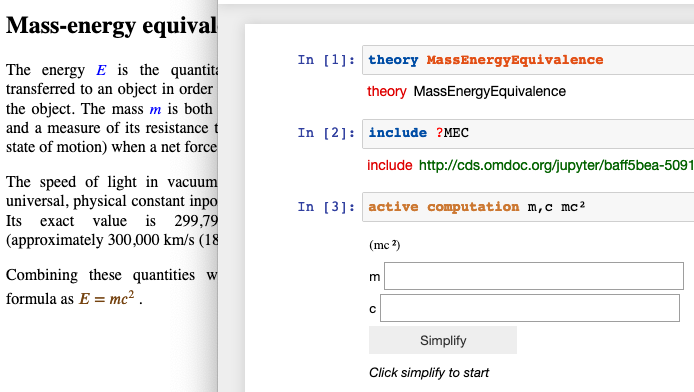
\includegraphics[width=8cm]{screenshots/emc}
\caption{The resulting Jupyter notebook}\label{fig:conversionNotebook}
\end{wrapfigure}

Figure~\ref{fig:conversionHTML} shows a (simplified) scientific HTML document (on the left) and an extract of it's source code (on the right). 
The document contains the equation $E=mc^2$. 
The user can use the context menu to trigger the notebook generation on this formula.

This scientific document is semantically annotated. 
Most notably, the formula that the user can interact with defines the variables that the user might want to interactively change using the \texttt{data-declares} attribute. 
Futhermore, the document contains a reference to an MMT context (using the \texttt{data-theory} attribute). 
This gives semantic meaning to the formula. 

The context menu is generated using JavaScript that picks up on these annotations.
Currently the author has to manually create the formula and context annotations, but we are working on a mechanism to automatically create it from the document context.
The data is then sent to our Jupyter installation using appropriate URL parameters. 

Figure~\ref{fig:conversionNotebook} shows the notebook created by our tool.
This notebook starts with an \texttt{include} declaration of the document context. 
These are generated by our tool to obtain a minimal standalone MMT theory in which the respective formula is well-formed. 
The notebook then directly instantiates the active computation widget we presented above using the parameters extracted from the document. 

In this demonstration we directly show the Jupyter Notebook to the user in a separate window. 
If desired, the notebooks can be easily uploaded to the Jupyter server, stored persistently in the repository server, or evaluated in a locally deployed version of the system per drag-and-drop.

%%% Local Variables:
%%% mode: latex
%%% mode: visual-line
%%% fill-column: 5000
%%% TeX-master: "paper"
%%% End:

%  LocalWords:  Jupyter ednote compactenum textsf texttt visualizations RupKohMue:fitgv17 nbdime centering fbox includegraphics NB-Mathhub compactitem oldpart vspace sciencedoc wrapfigure emc Futhermore
